 \documentclass[12pt,a4paper]{article}
\usepackage{amsmath}
\usepackage{amssymb}
\usepackage{epstopdf}
\usepackage{inputenc}
\usepackage{graphicx}
\usepackage{titletoc} 
\usepackage{fancyhdr}   
\usepackage[a4paper,pdftex]{geometry}	
\usepackage[english]{babel}
\usepackage{xcolor} 
\usepackage{enumerate}
\usepackage{fix-cm} 
\usepackage[notlof]{tocbibind}
\usepackage{amsmath}
\usepackage{listings}
\usepackage{float}
\usepackage{enumitem}
\usepackage{xcolor}
\usepackage{listings}
\definecolor{vgreen}{RGB}{104,180,104}
\definecolor{vblue}{RGB}{49,49,255}
\definecolor{vorange}{RGB}{255,143,102}
\renewcommand\lstlistingname{Appendix}
\renewcommand\lstlistlistingname{Appendix}

\makeatletter
\newcommand*\@lbracket{[}
\newcommand*\@rbracket{]}
\newcommand*\@colon{:}
\newcommand*\colorIndex{%
	\edef\@temp{\the\lst@token}%
	\ifx\@temp\@lbracket \color{black}%
	\else\ifx\@temp\@rbracket \color{black}%
	\else\ifx\@temp\@colon \color{black}%
	\else \color{vorange}%
	\fi\fi\fi
}
\makeatother

\usepackage{trace}

\usepackage{subcaption}
\begin{document}
	\begin{titlepage}
		\begin{center}
			
\includegraphics[scale=.4]{Figures/Cover}\\
			\vspace{1cm}
			\bf{ \large {Department of Computer Science and Technology} }
		\end{center}
		
		\vspace{4cm}
		\centering
		\textbf{\Huge Machine Learning}
		\vspace{.5cm}
		
		{\Large Homework 1}

		\vspace{4cm}
		
		\textbf{\LARGE Sahand Sabour}
		
		
		
		\vspace{0.5cm}
		
		{\large 2020280401}
		
		
		\vfill
		
	\end{titlepage}

	\section{Mathematics Basics}
	\subsection{Optimization}
	Use the Lagrange multiplier method to solve the following problem:
	\begin{align*}
		\underset{x_1, x_2}{\min} \qquad  x_1^2 +x_2^2-1 \\
		s.t. \quad x_1 +x_2-1=0 \\
		x_1-2x_2\geq 0
	\end{align*}
	\noindent \textbf{Solution:}
	\vspace{0.2cm}
	
	\noindent The Lagrangian equation can be written as $L(x_1, x_2, \lambda_1, \lambda_2)$, where $\lambda_1$ and $\lambda_2$ are the Lagrange multipliers. Therefore, Lagrangian function would be written as:
	\begin{align*}
		\mathcal{L}(x_1, x_2, \lambda_1, \lambda_2) = x_1^2 +x_2^2-1 - \lambda_1(x_1 +x_2-1)-\lambda_2(x_1-2x_2)
	\end{align*}
	Hence, we can have that:
	\begin{align*}
		\frac{\partial \mathcal{L}}{\partial x_1}=0 \quad => \quad 2x_1-\lambda_1-\lambda_2=0 \quad => \quad x_1^* = \frac{\lambda_1+\lambda_2}{2}\\
		\frac{\partial \mathcal{L}}{\partial x_2}=0 \quad => \quad 2x_2+\lambda_2+2\lambda_2=0 \quad => \quad x_2^* = \frac{\lambda_1-2\lambda_2}{2}
	\end{align*}
	
	\noindent Accordingly, using the above equations, we can expand and rewrite the Lagrangian equation as follows:
	\begin{align*}
		\mathcal{L}(\lambda_1, \lambda_2) = \frac{1}{4}\lambda_1^2+\frac{1}{2}\lambda_1\lambda_2+\frac{1}{4}\lambda_2^2 
		+\frac{1}{4}\lambda_1^2-\lambda_1\lambda_2+\lambda_2^2 \\
		-1 
		-\lambda_1^2+\frac{1}{2}\lambda_1\lambda_2+\lambda_1
		+\frac{1}{2}\lambda_1\lambda_2-\frac{5}{2}\lambda_2^2 \\
		= -\frac{1}{2}\lambda_1^2-\frac{5}{4}\lambda_2^2+\frac{1}{2}\lambda_1\lambda_2+\lambda_1-1 \qquad \quad
	\end{align*}
	Therefore, we can have that:
	\begin{align*}
	\frac{\partial \mathcal{L}}{\partial \lambda_1}=0 \quad => -\lambda_1+\frac{1}{2}\lambda_2+1=0 \\
	\frac{\partial \mathcal{L}}{\partial \lambda_2}=0 \quad => -\frac{5}{2}\lambda_2+\frac{1}{2}\lambda_1=0
	\end{align*}
	Solving the above two equations gives $\lambda_1=\frac{10}{9}$ and $\lambda_2 = \frac{2}{9}$. Accordingly, we use these values to obtain $x_1=\frac{2}{3}$ and $x_2=\frac{1}{3}$ based on the initial two derivations. Since (1) both Lagrange multipliers satisfy $\lambda\geq 0$; (2) $g(x)=x_1+x_2-1 = \frac{2}{3}+\frac{1}{3}-1=0$ and $h(x)=x_1-2x_2 = \frac{2}{3}-2(\frac{1}{3})=0\geq 0$; (3) $\lambda_2h(x) = \frac{2}{9}(\frac{2}{3}-2(\frac{1}{3}))=0 $; KKT conditions are satisfied and therefore, the solutions $x_1=\frac{2}{3}$ and $x_2=\frac{1}{3}$ are valid.
	
	
	
	
	\subsection{Stochastic Process}
	\noindent We toss a fair coin for a number of times and use H(head) and T(tail) to denote the two sides of the coin. Please compute the expected number of tosses we need to observe a first time occurrence of the following consecutive pattern
	\begin{center}
		H, T, T, ..., T
	\end{center}
	\vspace{-0.2cm}
	
	\noindent \textbf{Solution:}
	\vspace{0.2cm}
	
	\noindent Let x denote the number of tosses we need to get n consecutive turns of the same side (i.e n heads or n tails). For the first toss, if we get the side we want immediately, then the probability would be $\frac{1}{2}$. Otherwise, this turn is useless and the number of turns would be x+1. In the second toss, the probability of getting the order we want is $\frac{1}{2}\times\frac{1}{2}=\frac{1}{4}$ and the case that we don't get what we want, the number of turns would be x+2. This gives us the following sequence for the expected number of tosses before observing our desired pattern for a coin side:
	\begin{align*}
		x=\frac{1}{2}(x+1)+\frac{1}{4}(x+2)+\frac{1}{8}(x+3)+...
	\end{align*}
	
	\noindent Accordingly, solving the above equation gives $x_{S(n)}=2(2^n-1)$, where S is the side we want to observe n times. Hence, if we think of this problem as number of tosses to see one consecutive head and k consecutive tails, we would need $x_{H(1)}+x_{T(k)}=2(2^1-1)+2(2^k-1)= 2+2^{k+1}-2 =2^{k+1}$ tosses to observe this pattern.
	
	\section{SVM}
	Consider the regression problem with training data $\{(x_i, y_i)\}_{i=1}^N (x_i \in R^d, y_i \in R)$. $\epsilon<0$ denotes a fixed small value. Derive the dual problem of the following primal problem of linear SVM:
	\begin{align*}
		\underset{w, b, \xi, \hat{\xi}}{min}\quad \frac{1}{2}||w||^2\quad+\quad C\sum_{i=1}^{N}(\xi_i+\hat{\xi}_i)\\
		s.t.\quad y_i\quad \leq \quad w^Tx_i+b+\epsilon+\xi_i, i=1,...,N \\	
		y_i\quad \geq\quad w^Tx_i+b-\epsilon-\xi_i, i=1,...,N\\
		\xi_i\quad\geq\quad 0\quad\forall i=1,...,N\qquad\qquad\quad\quad\\
		\hat{\xi}_i\quad\geq\quad 0\quad\forall i=1,...,N\qquad\qquad\quad\quad
	\end{align*}
	\vspace{-0.8cm}
	
	\noindent \textbf{Solution:}
	\vspace{0.2cm}
	
	\noindent Let $a, c, d, \text{and } e \geq 0$ be the Lagrange multipliers. Then, the Lagrangian function would be
	\begin{align*}
		\mathcal{L}(w, b, \xi, \hat{\xi}, a, c, d, e) = \frac{1}{2}||w||^2 + C\sum_{i}(\xi_i+\hat{\xi}_i)-\sum_{i}a_i(w^Tx_i+b+\epsilon+\xi_i-y_i)\\-\sum_{i}c_i(y_i-w^Tx_i-b+\epsilon+\hat{\xi}_i)-\sum_{i}d_i\xi_i-\sum_{i}e_i\hat{\xi}_i \quad \quad
	\end{align*}
	
	\noindent Therefore, we can have that
	\begin{align}
		\frac{\partial \mathcal{L}}{\partial w} =\hat{w} -\sum_{i=1}^{N}a_ix_i + \sum_{i=1}^{N}c_ix_i=0 \quad giving \quad \hat{w}=\sum_{i=1}^{N}(a_i-c_i)x_i\\
		\frac{\partial \mathcal{L}}{\partial b} =-\sum_{i=1}^{N}a_ix_i+\sum_{i=1}^{N}c_ix_i = 0 \quad giving \quad \sum_{i}a_i-c_i= 0\quad\\
		\frac{\partial \mathcal{L}}{\partial \xi} = C1-\sum_{i}a_i-\sum_{i}d_i= 0\quad giving 
		\quad C = a+d\qquad \\
		\frac{\partial \mathcal{L}}{\partial \hat{\xi}} =C1+\sum_{i}c_i-\sum_{i}e_i= 0\quad giving 
		\quad C = c+e \qquad
	\end{align}
	
	\noindent Therefore, we initially expand the Lagrangian function as below
	\begin{align*}
	\mathcal{L}(w, b, \xi, \hat{\xi}, a, c, d, e) = 
	\frac{1}{2}||w||^2
	+ C\sum_{i}(\xi_i+\hat{\xi}_i)
	-\sum_{i}a_iw^Tx_i
	-\sum_{i}a_ib
	-\sum_{i}a_i\epsilon \\
	-\sum_{i}a_i\xi_i
	+\sum_{i}a_iy_i
	-\sum_{i}c_iy_i
	+\sum_{i}c_iw^Tx_i
	+\sum_{i}c_ib \qquad\\
	-\sum_{i}c_i\epsilon
	-\sum_{i}c_i\hat{\xi}_i
	-\sum_{i}d_i\xi_i-\sum_{i}e_i\hat{\xi}_i \qquad\qquad\qquad\qquad \\
	 = 
	\frac{1}{2}||w||^2
	+ C\sum_{i}(\xi_i+\hat{\xi}_i)
	-\sum_{i}(a_i-c_i)w^Tx_i\qquad\qquad \quad\\
	-\sum_{i}(a_i-c_i)b
	-\sum_{i}(a_i+c_i)\epsilon
	-\sum_{i}(a_i+d_i)\xi_i\qquad\qquad\\
	+\sum_{i}(a_i-c_i)y_i
	-\sum_{i}(c_i+e_i)\hat{\xi}_i\qquad\qquad \qquad\qquad\qquad
	\end{align*}
	
	\noindent Then, using equations 5-8 ,we can write the Lagrangian function as 
	\begin{align*}
	\mathcal{L}(w, b, \xi, \hat{\xi}, a, c, d, e) = 
	\frac{1}{2}||w||^2-\hat{w}w^T-b(0)-\epsilon\sum_{i}(a_i+c_i)+\sum_{i}(a_i-c_i)y_i\\
	+ C\sum_{i}(\xi_i+\hat{\xi}_i)
	-\sum_{i}(a_i+d_i)(\xi_i+\hat{\xi}_i)\qquad\qquad\qquad \quad\\ =-\frac{1}{2}||w||^2-\epsilon\sum_{i}(a_i+c_i)+\sum_{i}(a_i-c_i)y_i\qquad\qquad \quad
	\end{align*}

	\noindent Hence, the dual optimization problem would be
	\begin{align*}
		\underset{a, c}{argmax}-\frac{1}{2}\sum_{i}\sum_{j}(a_i-c_i)(a_j-c_j)x_i^Tx_j-\epsilon\sum_{i}(a_i+c_i)+\sum_{i}(a_i-c_i)y_i \\
		s.t \qquad \sum_{i}(a_i-c_i)=0\qquad\qquad\qquad\qquad\qquad\qquad\\
		0 \leq a_i, c_i \leq C\qquad\qquad\qquad\qquad\qquad\qquad
	\end{align*}
	
	\section{Deep Neural Networks}
	
	\noindent To make neural networks work well in practice is not easy in general, since there are too many hyper-parameters to tune such as the choice of the number of hidden layers, the activation function, the learning rate and so on. Besides some general guidelines (some standard techniques which are useful at most cases such as dropout, data augmentation), experience is of great importance.
	
	\noindent Though a beginner may often be confused with them, luckily, there are some software available on the internet to help you build up a good sense on tuning neural networks. In this problem, you need to train the neural networks with different choices of hyper-parameters from the following link - A Neural Network Playground (you may need a VPN) - and answer the following questions:
	
	\begin{enumerate}
		\item Identify the best configuration you find for different problems and datasets. Here you only need to list you configuration for the bottom-right dataset of the classification problem.
		
		\item List your findings that how the learning rate, the activation function, the number of hidden layers and the regularization influence the performance and convergence rate.
	\end{enumerate}
	\newpage
	\noindent \textbf{Solution:}
	\begin{enumerate}
		\item The values for the best configuration are provided respectively below:
			\vspace{-0.2cm}
		\begin{figure}[H]
			\centering
			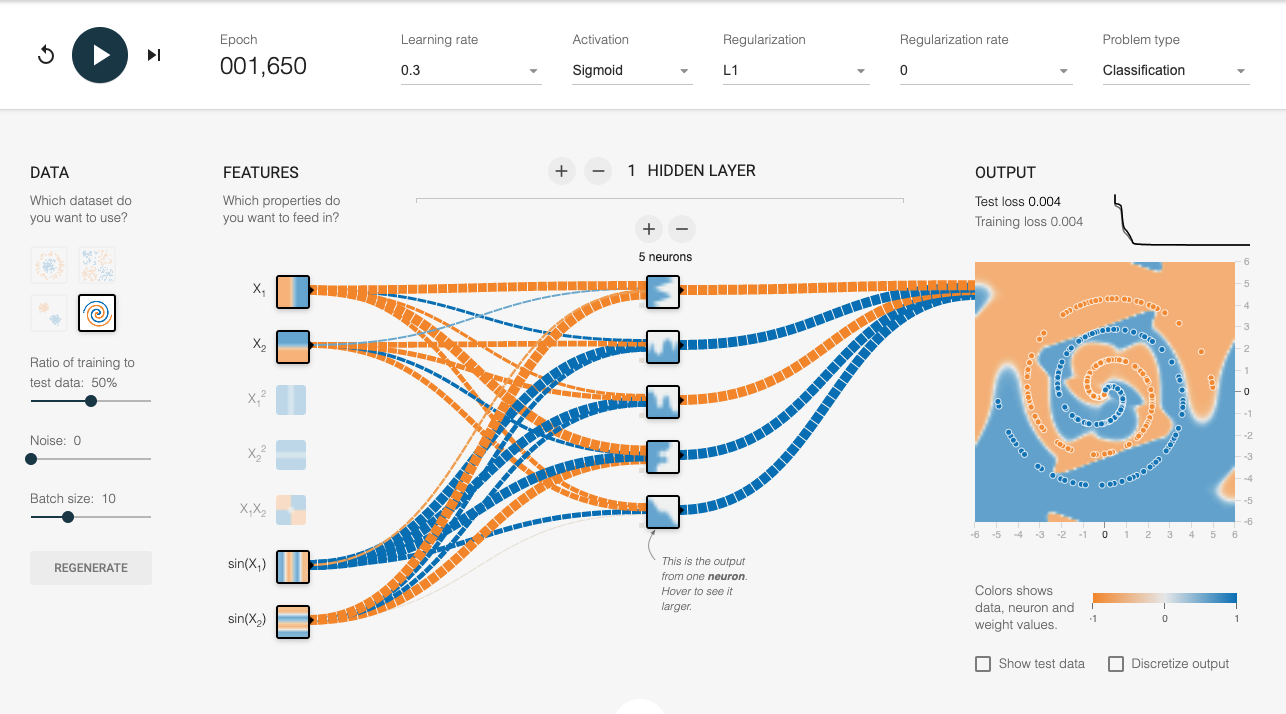
\includegraphics[width=13cm, height=6.5cm]{Figures/config}
			\caption{Best playground configuration}
		\end{figure}
	
			\vspace{-0.7cm}
		\begin{table}[H]
			\begin{center}
				\begin{tabular}{|c|c|c|c|c|}
					\hline
					Learning Rate & Activation & Regularization&Features & Hidden parameters \\ \hline
					0.03 & Sigmoid&None&$x_1, x_2, sin(x_1), sin(x_2)$&1 layer - 5 neurons\\ \hline
				\end{tabular}
			\end{center}
		\vspace{-0.5cm}
			\caption{Best configuration parameters}
		\end{table}
		
		\vspace{-0.7cm}
		\item The analyzed parameters and their influence for the performance and convergence rate are discussed respectively below:
	
		\noindent \textbf{\small Learning Rate}: as the name suggests, the learning rate relates to the rate at which the model learns; i.e. the amount of correction that is applied to weights with each training example. 
			\begin{figure}[H]
			\centering
			\begin{subfigure}[H]{0.2\textwidth}
				\centering
				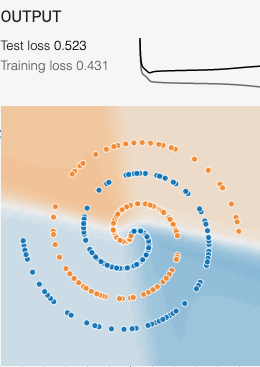
\includegraphics[width=\textwidth]{Figures/lr/lol0}
				\caption{$lr=0.01$}
			\end{subfigure}
			\begin{subfigure}[H]{0.2\textwidth}
				\centering
				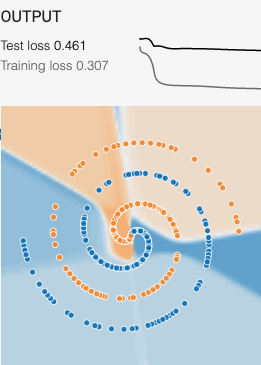
\includegraphics[width=\textwidth]{Figures/lr/lol}
				\caption{$lr=0.1$}
			\end{subfigure}
			\begin{subfigure}[H]{0.2\textwidth}
				\centering
				
\includegraphics[width=\textwidth]{Figures/lr/1}
				\caption{$lr=1$}
			\end{subfigure}
			\begin{subfigure}[H]{0.2\textwidth}
				\centering
				
\includegraphics[width=\textwidth]{Figures/lr/10}
				\caption{$lr=10$}
			\end{subfigure}
			\caption{Four different learning rates}
		\end{figure}
		\vspace{-0.5cm}
		\noindent Hence, smaller values of the learning rate may result in a considerably slow convergence while larger values of learning rate may result in over-shooting as the local minima point may be missed due to large changes. Therefore, the learning rate should be set to a small enough value to ensure that it does not miss its convergence point, but a large enough value to reach convergence in a reasonable amount of time (i.e. avoid slow convergence). In practice, the learning set is initially rate is set to 0.01 and may be slightly modified depending on the given application. This is further shown by the above illustrations as too small and too large learning rates led to increased loss.
		
		\noindent \textbf{\small Activation Function}: this is a function that determines the final output of the model and it could either a linear or a nonlinear function. Accordingly, since linear functions only work with linear data, they are insufficient for producing nonlinear outputs. Since activation functions have different complexities, execution times, etc., a fitting activation function should be chosen based on the characteristics of the data for which we are building the model. 
		\begin{figure}[H]
			\centering
			\begin{subfigure}[H]{0.2\textwidth}
				\centering
				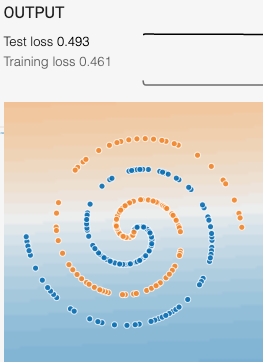
\includegraphics[width=\textwidth]{Figures/activation/linear}
				\caption{$Linear$}
			\end{subfigure}
			\begin{subfigure}[H]{0.2\textwidth}
				\centering
				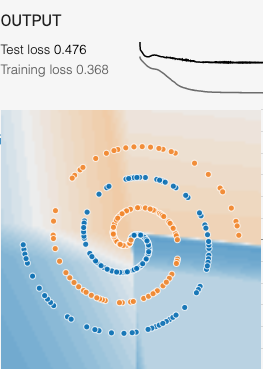
\includegraphics[width=\textwidth]{Figures/activation/relu}
				\caption{$Relu$}
			\end{subfigure}
			\begin{subfigure}[H]{0.2\textwidth}
				\centering
				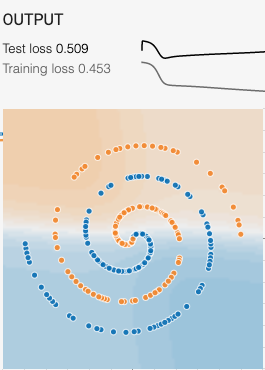
\includegraphics[width=\textwidth]{Figures/activation/sigmoid}
				\caption{$Sigmoid$}
			\end{subfigure}
			\begin{subfigure}[H]{0.2\textwidth}
				\centering
				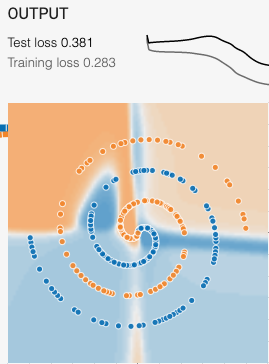
\includegraphics[width=\textwidth]{Figures/activation/tanh}
				\caption{$Tanh$}
			\end{subfigure}
		\vspace{-0.1cm}
			\caption{Four different activation functions}
		\end{figure}
		
		\vspace{-0.5cm}
		
		\noindent \textbf{\small Number of Hidden Layers}: the number of hidden layers determines the amount of information available for the model for producing the output. 
		\begin{figure}[H]
			\centering
			\begin{subfigure}[H]{0.2\textwidth}
				\centering
				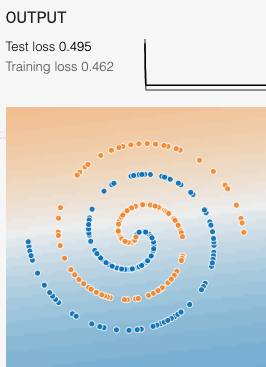
\includegraphics[width=\textwidth]{Figures/hidden/0}
				\caption{0 layers}
			\end{subfigure}
			\begin{subfigure}[H]{0.2\textwidth}
				\centering
				
\includegraphics[width=\textwidth]{Figures/hidden/1}
				\caption{1 layers}
			\end{subfigure}
			\begin{subfigure}[H]{0.2\textwidth}
				\centering
				
\includegraphics[width=\textwidth]{Figures/hidden/2}
				\caption{2 layers}
			\end{subfigure}
			\begin{subfigure}[H]{0.2\textwidth}
				\centering
				
\includegraphics[width=\textwidth]{Figures/hidden/3}
				\caption{3 layers}
			\end{subfigure}
		\vspace{-0.1cm}
			\caption{Four different number of hidden layers}
		\end{figure}
		\vspace{-0.5cm}
		\noindent Hence, too few hidden layers may not provide enough information for the model to produce a reasonable output, which results in under-fitting. If we implement too many hidden layers, there would be too much information for the model to process, which results in over-fitting as there may not be enough training examples to properly train a model of this scale. As demonstrated in the above figures, 2 hidden layers showed satisfactory results. However, the number of hidden neurons plays an important role in the results likewise.
		
		\noindent \textbf{\small Regularization}: the main usage of regularization is to add a penalty term to the change of weights as a means of avoiding over-fitting. The two generally used types of regularization are L1 and L2, which both follow the similar structure for the cost function: loss + regularization term. However, the regularization term in L1 is $\frac{\lambda}{2m}\sum||w||$ ($\frac{\lambda}{2m}$ being the regularization rate) whereas it is $\frac{\lambda}{2m}\sum||w||^2$ in L2. Therefore, L1 tends to move the weights to 0 whereas L2 focuses on decreasing the weights evenly, which makes L1 better for feature selection tasks and L2 useful in tasks where a number of features are dependent on one another. The figures below display the results obtained by both the L1 and L2 regularization methods with respective different regularization rates. Hence, it can be observed that for the given dataset, a rate of 0.003 would be satisfactory with L2 regularization performing better.
		\begin{figure}[H]
			\centering
			\begin{subfigure}[H]{0.2\textwidth}
				\centering
				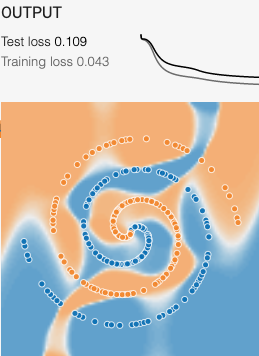
\includegraphics[width=\textwidth]{Figures/reg/L0001}
				\caption{L1 - 0.001}
			\end{subfigure}
			\begin{subfigure}[H]{0.2\textwidth}
				\centering
				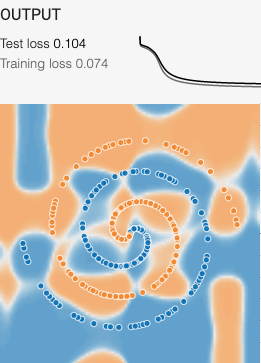
\includegraphics[width=\textwidth]{Figures/reg/L0003}
				\caption{L1 - 0.003}
			\end{subfigure}
			\begin{subfigure}[H]{0.2\textwidth}
				\centering
				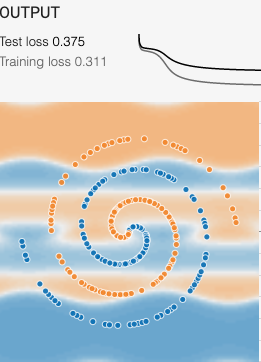
\includegraphics[width=\textwidth]{Figures/reg/L001}
				\caption{L1 - 0.01}
			\end{subfigure}
			\begin{subfigure}[H]{0.2\textwidth}
				\centering
				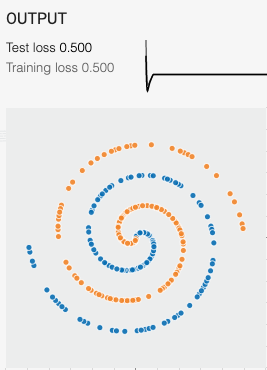
\includegraphics[width=\textwidth]{Figures/reg/L01}
				\caption{L1 - 0.1}
			\end{subfigure}
		\end{figure}
		\vspace{-0.7cm}
			\begin{figure}[H]
			\centering
			\begin{subfigure}[H]{0.2\textwidth}
				\centering
				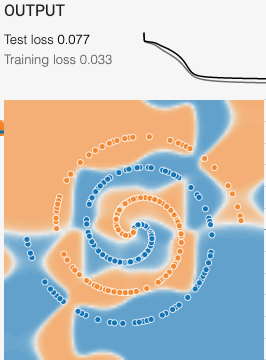
\includegraphics[width=\textwidth]{Figures/reg/L20001}
				\caption{L2 - 0.001}
			\end{subfigure}
			\begin{subfigure}[H]{0.2\textwidth}
				\centering
				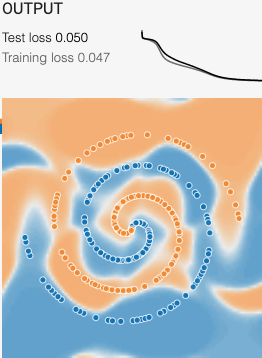
\includegraphics[width=\textwidth]{Figures/reg/L20003}
				\caption{L2 - 0.003}
			\end{subfigure}
			\begin{subfigure}[H]{0.2\textwidth}
				\centering
				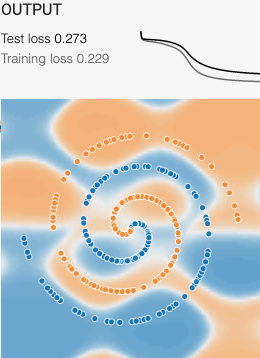
\includegraphics[width=\textwidth]{Figures/reg/L2001}
				\caption{L2 - 0.01}
			\end{subfigure}
			\begin{subfigure}[H]{0.2\textwidth}
				\centering
				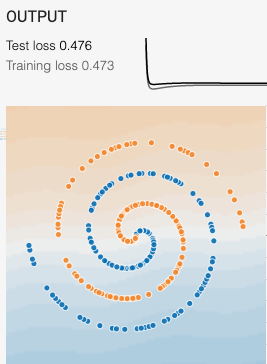
\includegraphics[width=\textwidth]{Figures/reg/L201}
				\caption{L2 - 0.1}
			\end{subfigure}
			\vspace{-0.1cm}
			\caption{Different regularization implementations}
		\end{figure}
		\vspace{-0.5cm}
		
	\end{enumerate}
	
	\newpage
	\section{IRLS for Logistic Regression}
	
	\noindent \textbf{Solution:}
	\vspace{0.2cm}
	
	\noindent \textbf{1. Data pre-processing:}
	\vspace{0.2cm}
	
	\noindent The provided datasets follows the below format:
	\begin{center}
		Label [feature id]:[feature] [feature id]:[feature] ......
	\end{center}
	where we have 123 features ($x$) in total, 32,561 samples for testing and 16,281 samples for training. Initially, an extra feature ($x_0$) known as the bias would be added, giving 124 features for each sample. Accordingly, since the labels for the provided samples are either -1 or 1, the label of all -1 samples are changed to 0 to make this a binary classification task.
	
	\vspace{0.4cm}
	\noindent \textbf{2. Weight update rule with L2 regularization:}  
	\vspace{0.2cm}
	
	\noindent By Newton's method, we aim to maximize the following
	\begin{align}
		\mathcal{L}(w) = \sum_{i}[y_iw^Tx_i-log(1+exp(w^Tx_i))]
	\end{align}
	
	\vspace{-0.2cm}
	\noindent By adding L2-regularization to the above equation, we get
	\begin{align}
	\mathcal{L}(w) = \sum_{i}[y_iw^Tx_i-log(1+exp(w^Tx_i))] - \frac{\lambda}{2}||w||^2_2
	\end{align}
	
	\vspace{-0.2cm}
	\noindent Accordingly, we need to find $w^*$ such that 
	\begin{align}
	\nabla_w\mathcal{L}(w^*) = \sum_{i}(y_i-\mu_i)x_i - \lambda w^*=0
	\end{align}
	
	\vspace{-0.2cm}
	\noindent The hessian matrix ($	H = \nabla^2_w\mathcal{L}(w)|_{w_t} = \nabla_w[\nabla_w\mathcal{L}(w)]^T$) would be
	\begin{align}
		\nabla_w[\sum_{i}(y_i-\mu_i)x^T - \lambda w^T]= -\sum_i\mu_i(1-\mu_i)x_ix^T_i  - \lambda = -XRX^T - \lambda I
	\end{align}
	
	\vspace{-0.2cm}
	\noindent Where $R_{ii}= \mu_i(1-\mu_i)$. Therefore, the weight update rule ($w_{t+1} \leftarrow w_t - H^{-1}\nabla_w\mathcal{L}(w)|_{w_t}$) would be as follows
	\begin{align}
		w_{t+1}\leftarrow w_t - [(-XRX^T - \lambda I)^{-1}][X^T(y_i-\mu_i) - \lambda w_t]
	\end{align}
	
	\vspace{-0.2cm}
	\noindent However, it should be noted that by getting closer to the point of convergence, $R$ slowly converges to 0, which causes the hessian matrix to be non-invertable. Hence, the inverse of H should be changed to its pseudo-inverse ($H^+$).
	
	\newpage
	\noindent \textbf{3. Data analysis:}
	\vspace{0.2cm}
	
	\noindent Initially, in order to find a beneficial value of $\lambda$ the training data is split into 10 folds (k=10). Accordingly, for a given array of lambda values ({0.01, 0.1, 1, 2, 5, 10, 20, 50, 100}), one of the folds is used as the testing data while the remaining 9 folds are used for training. The model would be trained for 10 epochs, and each of the 10 folds would be used once to test the model. Consequently, the average mean squared error (MSE) for each value of $\lambda$ during different folds and epochs was recorded and is provided in the below chart.
	
	\vspace{-0.6cm}
	\begin{figure}[H]
		\centering
		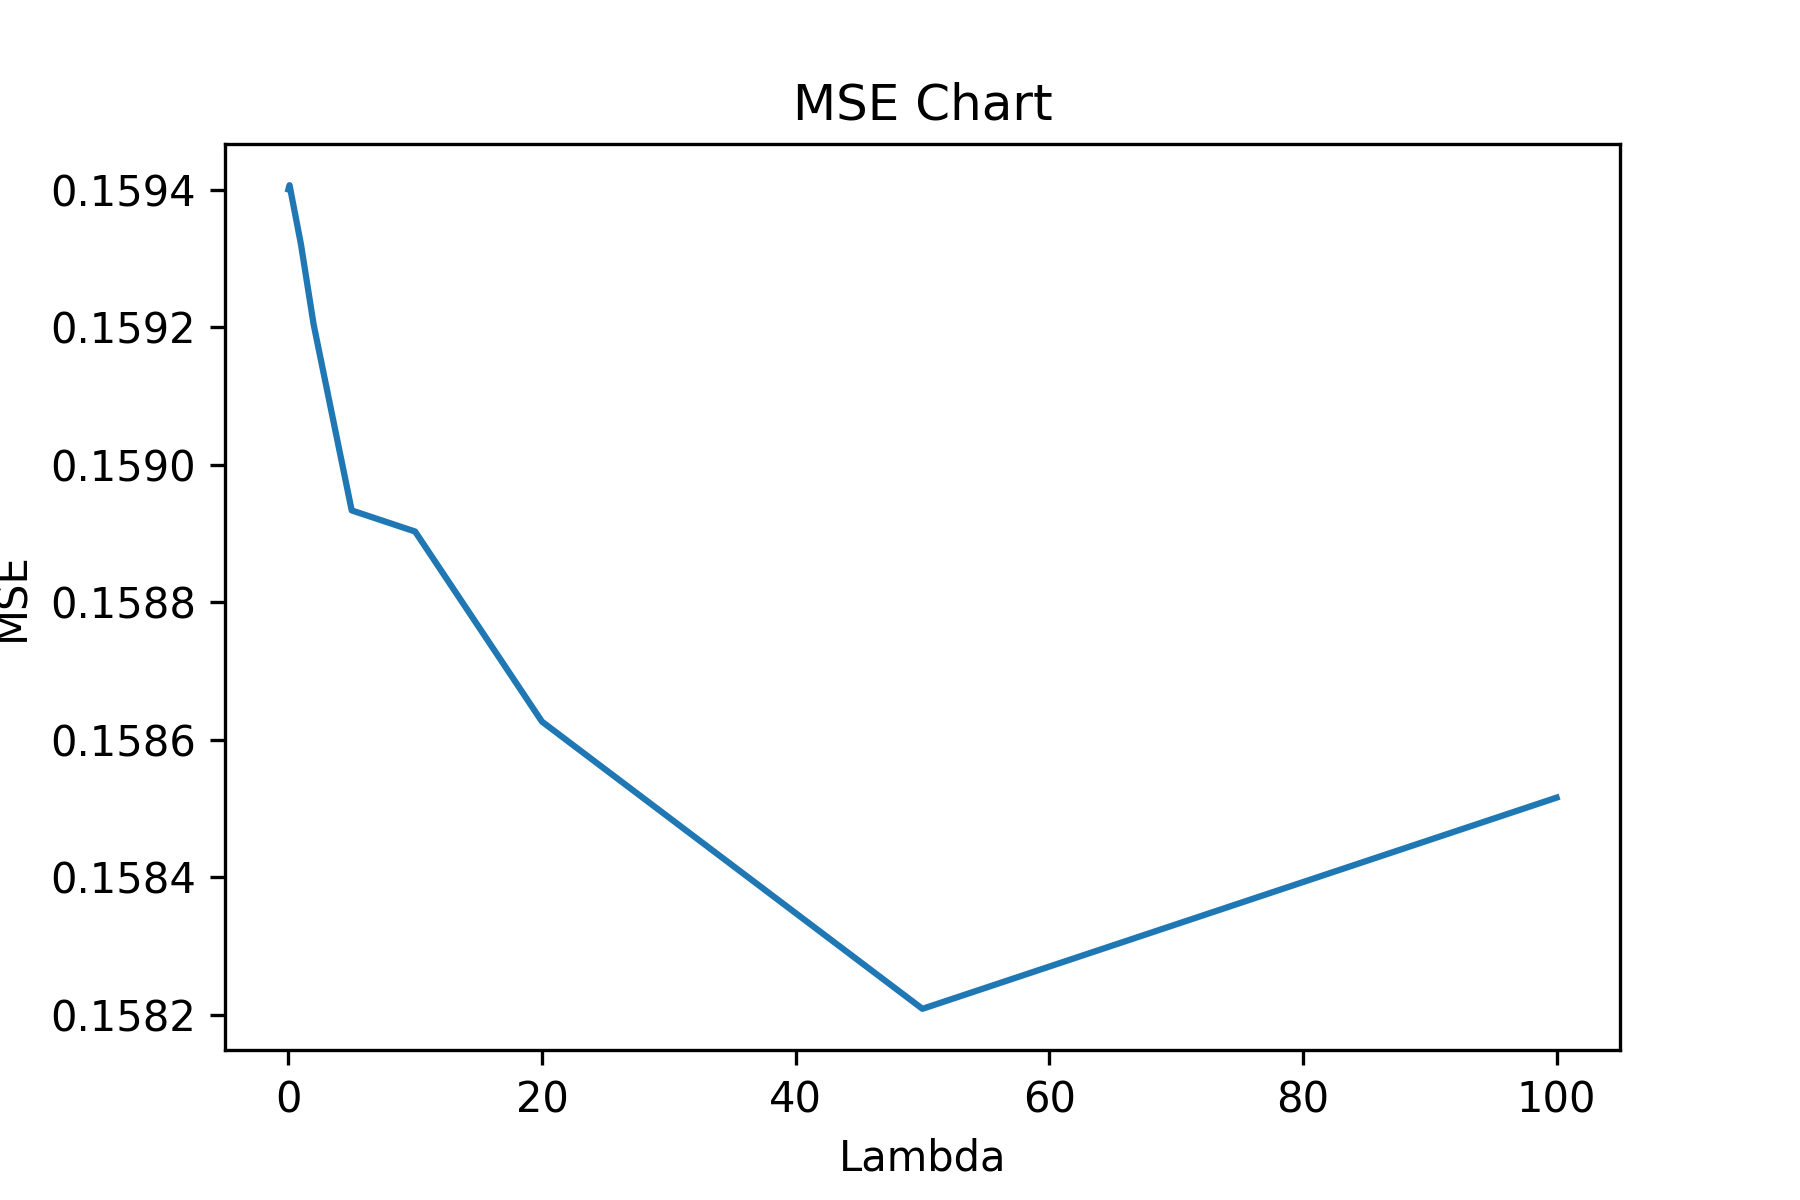
\includegraphics[scale=.63]{Figures/MSE}
		\caption{MSE chart for different values of $\lambda$}
	\end{figure}

	\vspace{-0.3cm}
	\noindent Consequently, as $\lambda = 50$ produced the lowest MSE in cross-validation, $\lambda$ for L2-regularization was set to this value. The following two figures illustrate the accuracy chart for the training and testing data for both normal and regularized logistic regressions respectively.

	\vspace{-0.4cm}
	\begin{figure}[H]
		\centering
		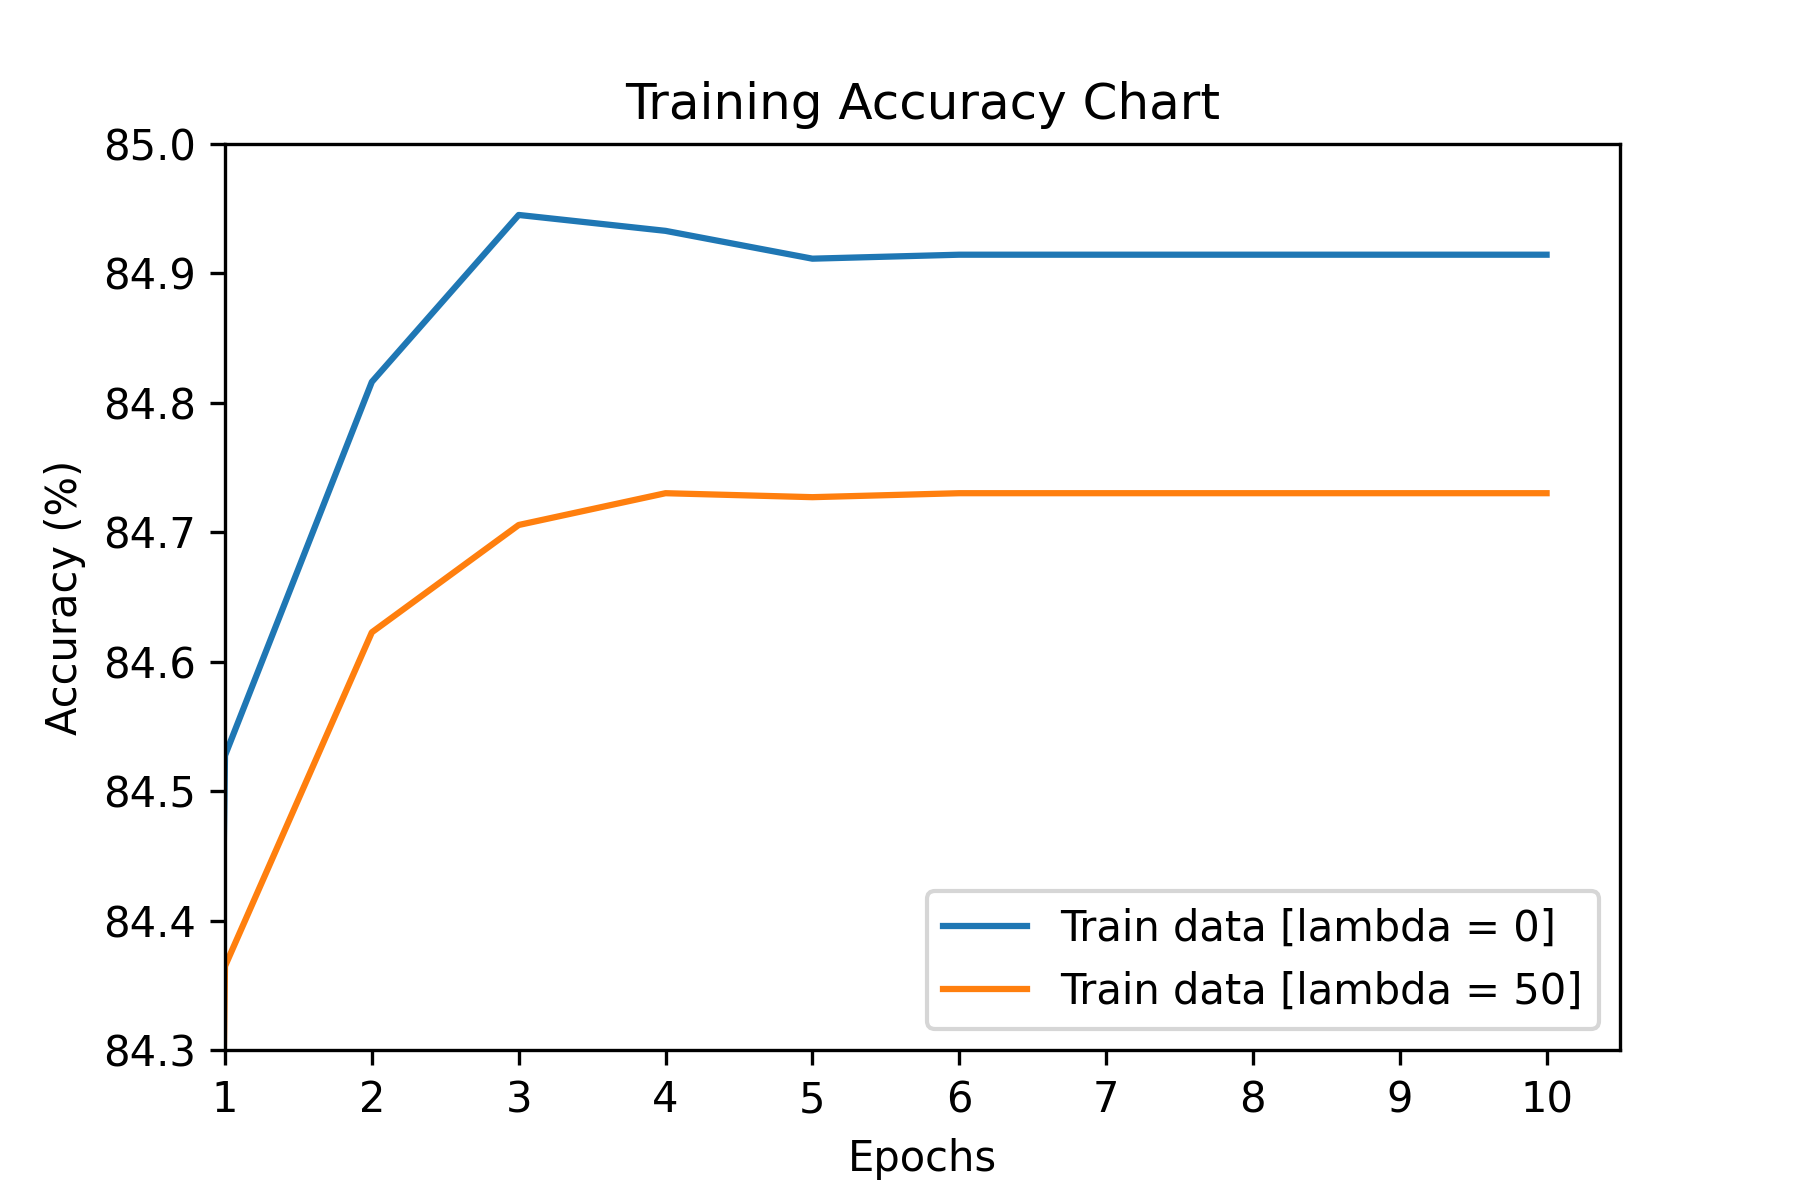
\includegraphics[scale=.63]{Figures/Acc_train}
		\caption{Accuracy chart for training data}
	\end{figure}
	
	\vspace{-0.6cm}
	\begin{figure}[H]
		\centering
		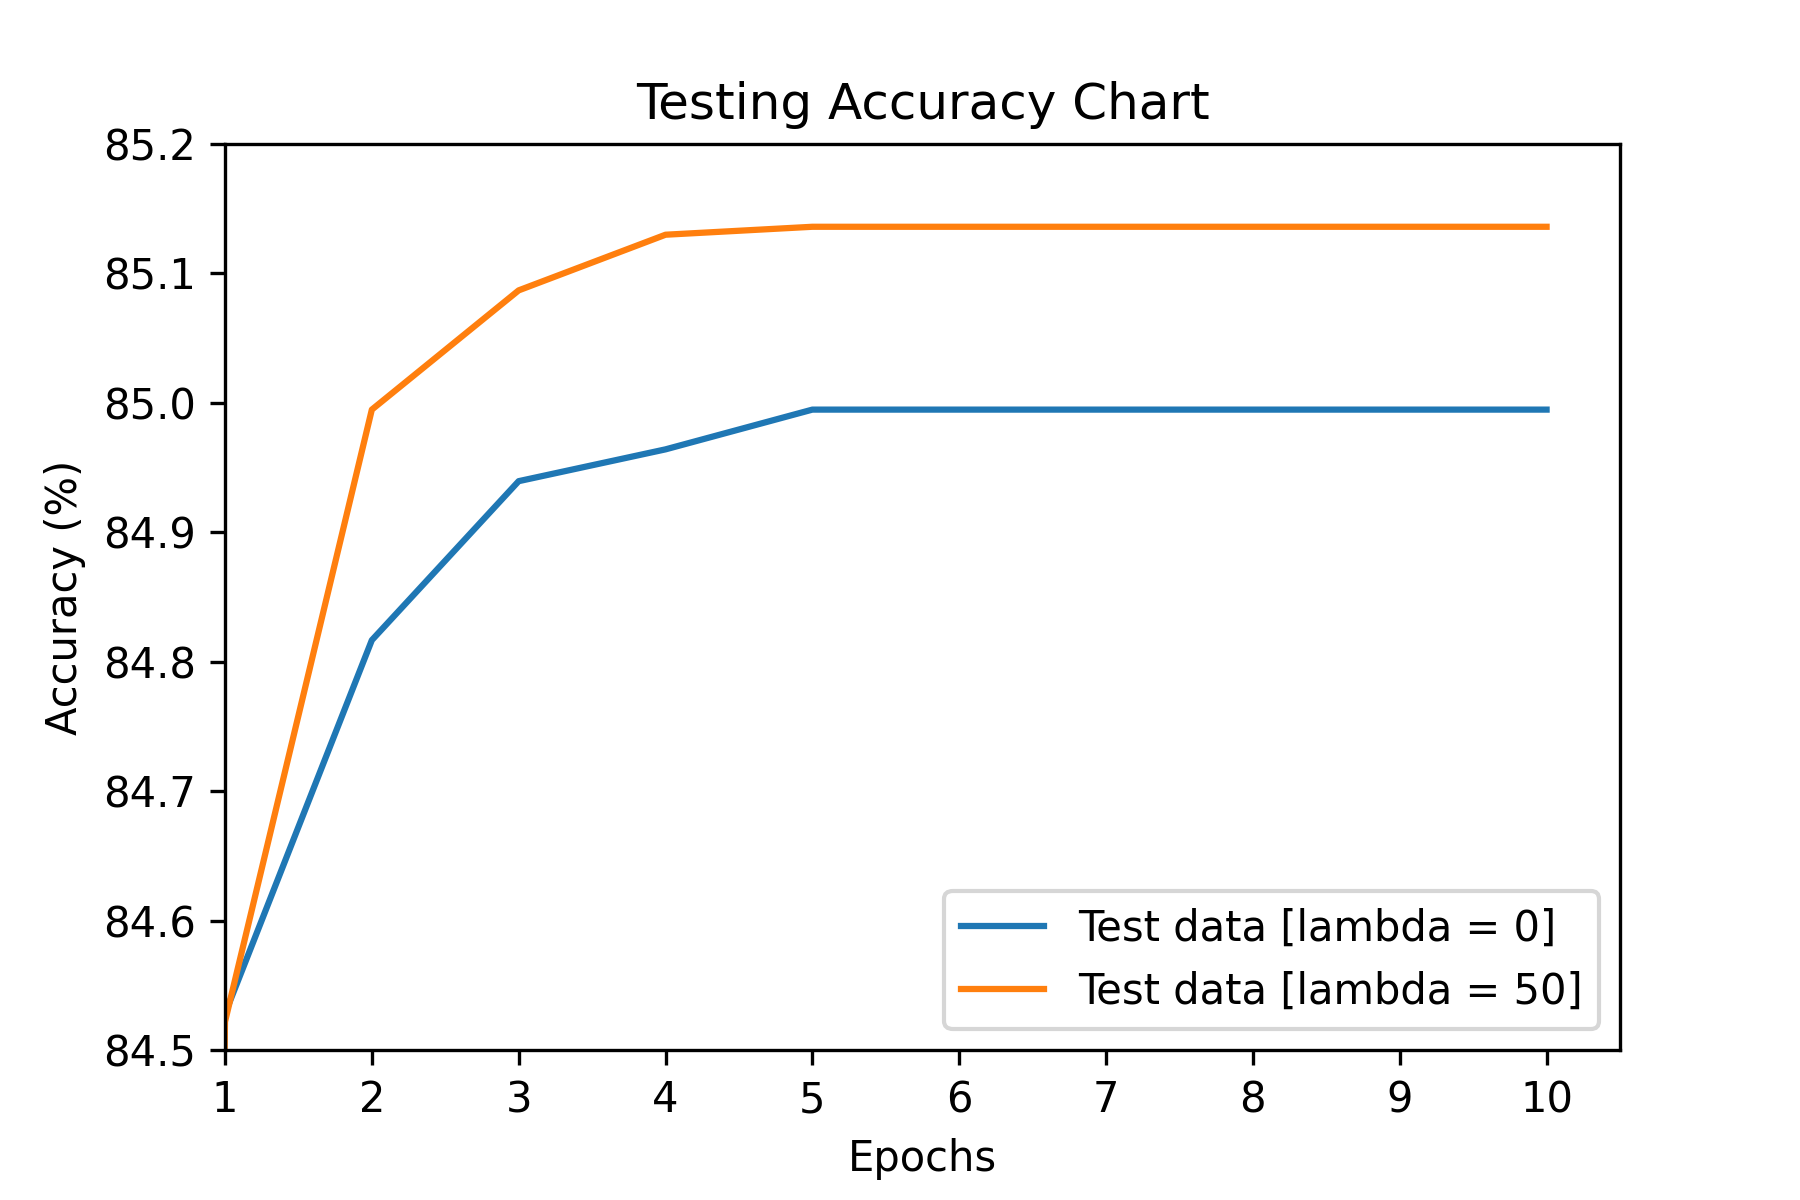
\includegraphics[scale=.63]{Figures/Acc_test}
		\caption{Accuracy chart for testing data}
	\end{figure}
	
	\vspace{-0.4cm}
	\noindent According to the above figures, both types of logistic regression converge nearly at the same number of epochs (=5). In addition, it can be seen that by regularization, the model achieves a lower accuracy on the training data while experiencing an increased accuracy with the test data. Therefore, it can be postulated that the regularized model would be able to generalize its predictions comparatively better than the normal logistic regression model. 
	
	\vspace{-0.4cm}
	\begin{figure}[H]
		\centering
		\begin{subfigure}[H]{0.45\textwidth}
			\centering
			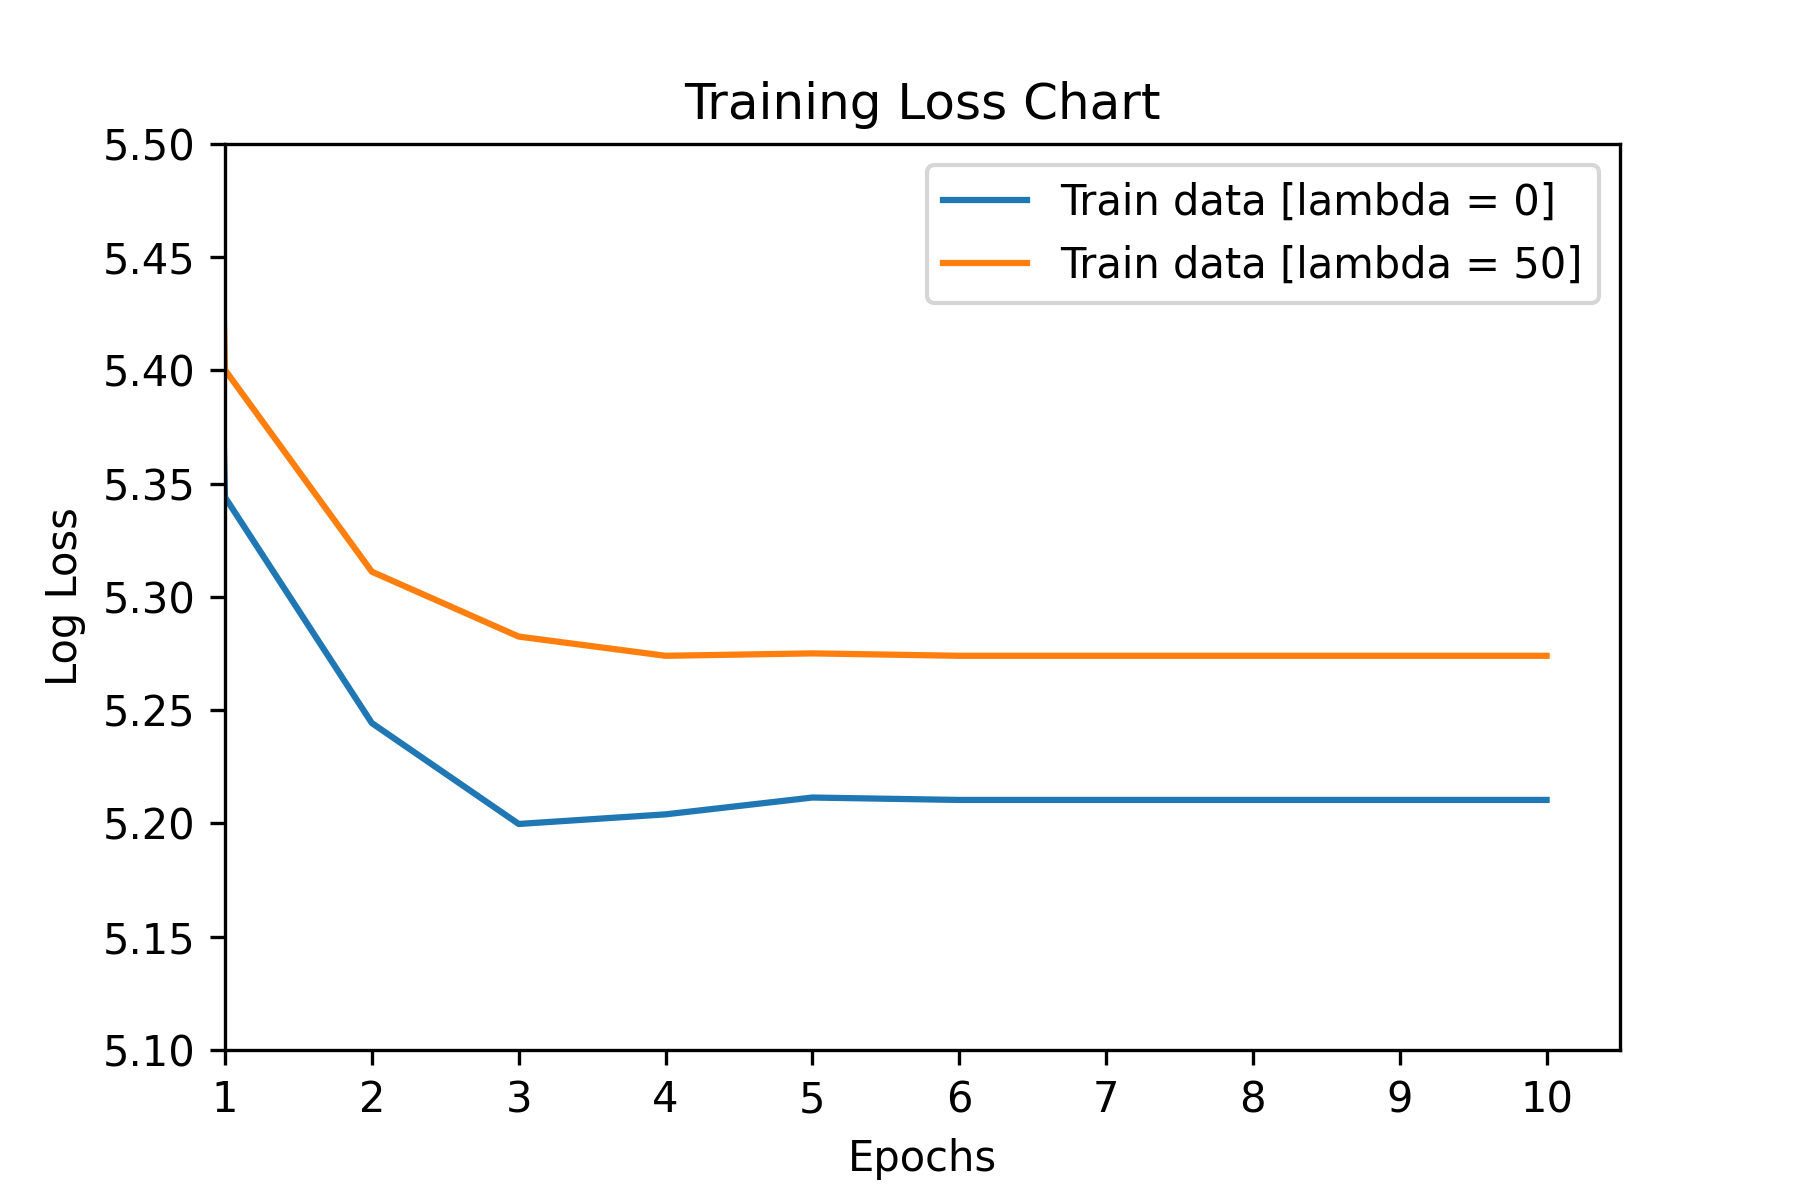
\includegraphics[width=1.2\textwidth]{Figures/Loss_train}
		\end{subfigure}
	\hfill
		\begin{subfigure}[H]{0.45\textwidth}
			\centering
			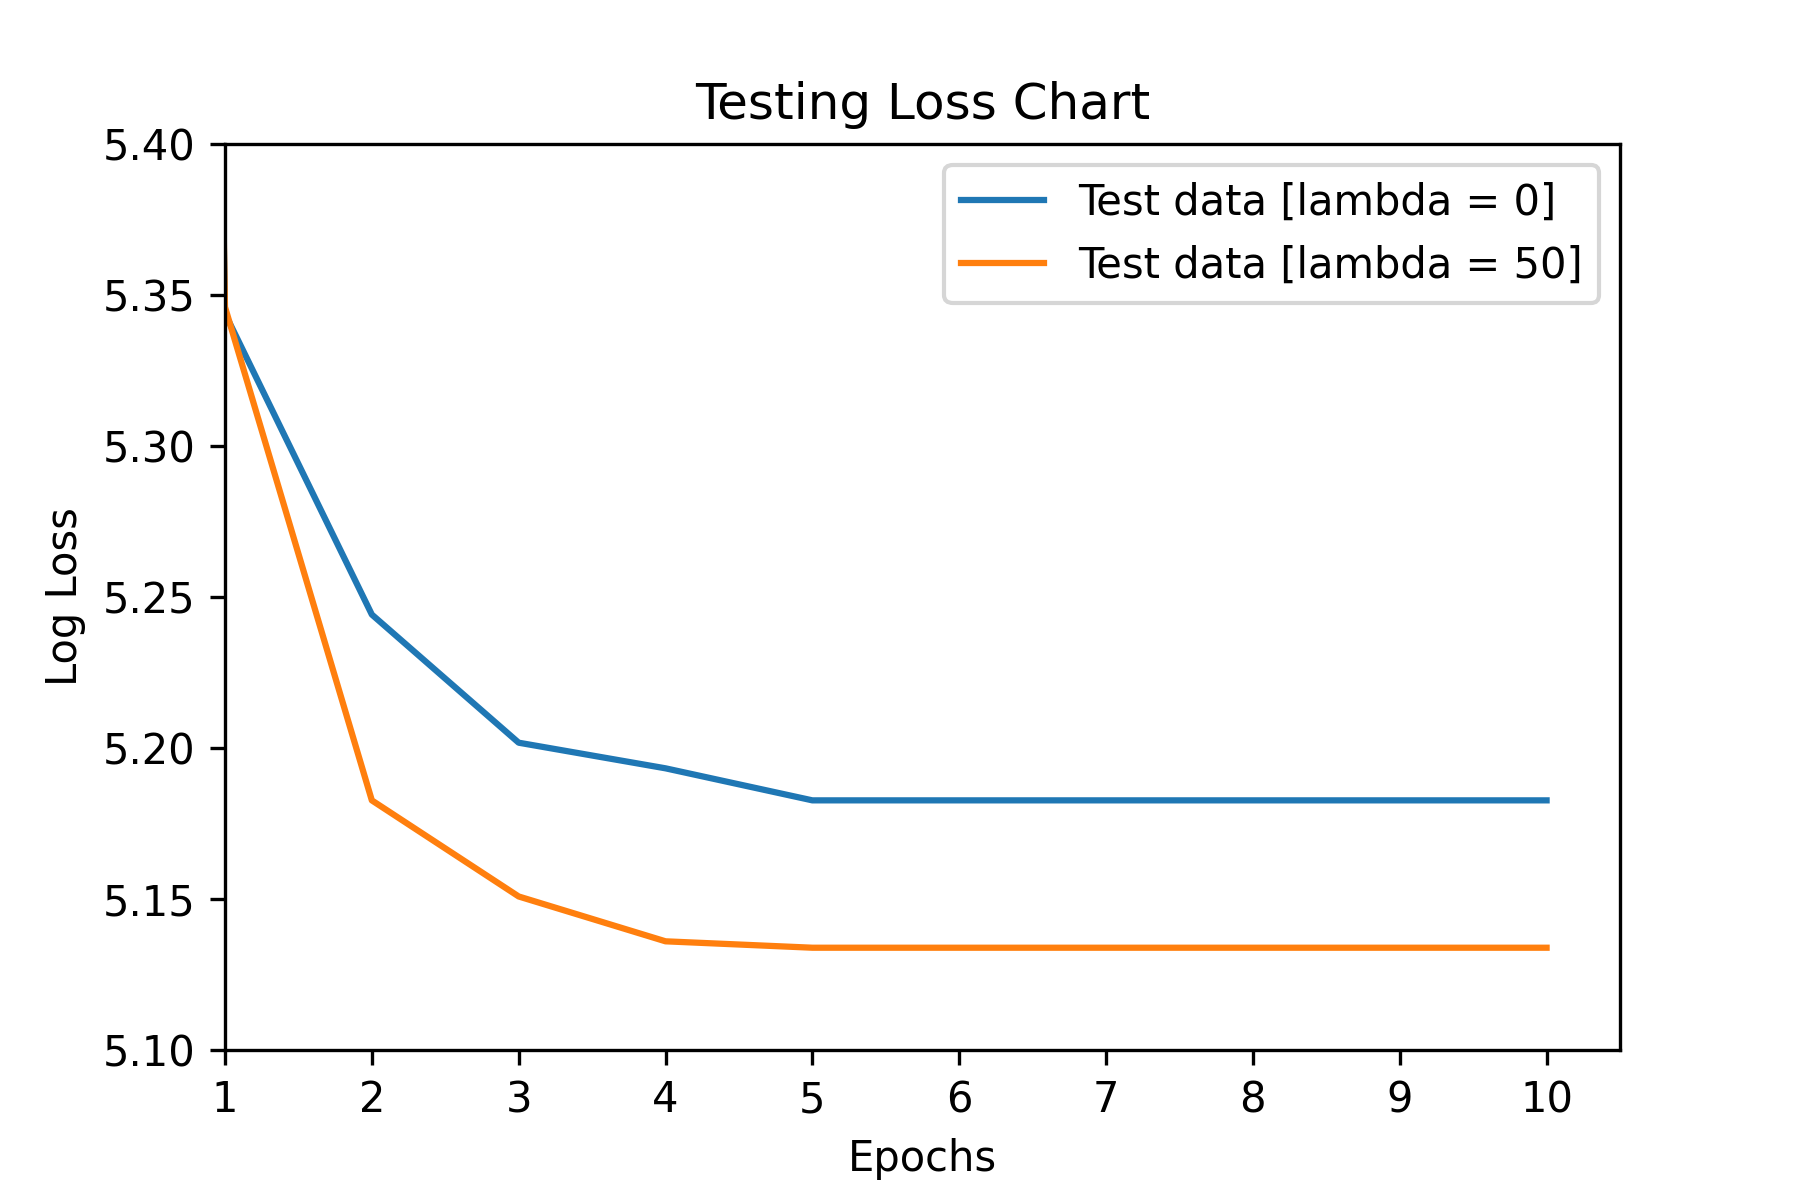
\includegraphics[width=1.2\textwidth]{Figures/Loss_test}
		\end{subfigure}
		\vspace{-0.1cm}
		\caption{Loss charts for training and testing data}
	\end{figure}
	
	\vspace{-0.4cm}
	\noindent Moreover, the logarithmic loss for both training and testing data was recorded during each epoch likewise. Figures 10 and 11 demonstrate the obtained results. As shown in the figures, similar to the recorded values of accuracy, the calculated loss for the training data was lower for the normal logistic regression model while the regularized model experienced less loss on the testing data. Hence, the previously drawn conclusion, which stated that the regularized model is able to perform better generalization, still stands.
	
\end{document}